\chapter{Antrenament}
\label{chapter4}
\section{Rețele MLP}

Primele experimente pe care le-am efectuat au fost efectuate folosind imaginile din care am extras ochii, pe care i-am convertit în imagini alb-negru (binary threshold), așa cum a fost menționat în prima parte a secțiunii de procesare de date\ref{data-processing:eyes}.
Fiecare ochi a fost redimensionat la 60x30 pixeli apoi au fost uniți orizontal, formând o imagine alb-negru de dimensiune 120x30 pixeli.
De asemenea, am etichetat fiecare imagine cu numărul celulei în care se uita utilizatorul, conform dimensiunii grilei folosite\ref{grid-example}.
Scopul a fost de a prezice, pentru imagini noi, numărul acelei celule.
Iată prima arhitectură pe care am încercat-o:

\begin{lstlisting}[language=Python, caption=Arhitectura MLP]
model = Sequential([
    Dense(100, input_shape=(n,), kernel_initializer='glorot_uniform'),
    Dropout(0.5),
    ReLU(),
    Dense(128, kernel_initializer='glorot_uniform'),
    Dropout(0.5),
    ReLU(),
    Dense(64, kernel_initializer='glorot_uniform'),
    # Dropout(0.5),
    ReLU(),
    Dense(Config.grid_size * Config.grid_size, activation='softmax')
])
\end{lstlisting}

\paragraph{Important}
Pentru primele experimente din această secțiune am folosit doar imaginile în care utilizatorul se uita în colțurile ecranului.
De exemplu, pentru o grilă de dimensiune 3x3, am ales doar imaginile în care eticheta corespunzătoare a imaginii este $0, 2, 6$ sau $8$.
Ultima mențiune este că datele de antrenament reprezintă $80\%$ din mulțimea totală de date, restul fiind date de testare.

\begin{center}
    \begin{tabular}{ c | c | c | c | c | c | c }
        \hline
        Experiment & Dim. grilă & Nr. imagini & Epoci & Optimizator & Rată învățare & Batch size \\ 
        \hline
        1 & 2x2 & 2184 & 300 & Adam & 0.001 & 32 \\
        \hline
        2 & 3x3 & 1247 & 300 & Adam & 0.001 & 32 \\
        \hline
        3 & 4x4 & 711 & 300 & Adam & 0.001 & 32 \\
        \hline
    \end{tabular}
\end{center}

Experimentele 2 și 3 au beneficiat de mai puține imagini de antrenament deoarece, dimensiunea grilei fiind mai mare, imaginile sunt mai dispersate și fiecare celulă are mai puține imagini corespunzătoare ei.
Evident, pentru o grilă 2x2, fiecare imagine se află intr-o celulă din colț (fiind doar 4), deci au fost folosite toate imaginile.

Primul rezultat pe care l-am constatat a fost că doar primul model putea prezice bine zona în care mă uitam.
Rețeaua MLP se descurca cu atât mai bine cu cât deschideam ochii mai mult, întrucât putea realiza mai bine conturul ochiului și să delimiteze pupila.

\begin{figure}[ht]
    \centering
    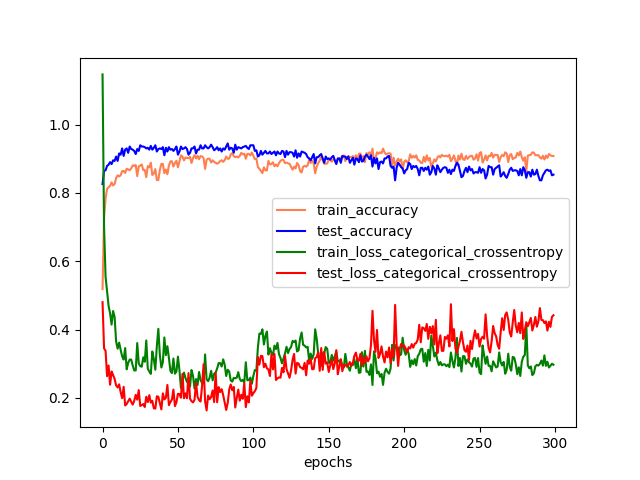
\includegraphics[width=0.49\textwidth]{graphs/model_1.png}
    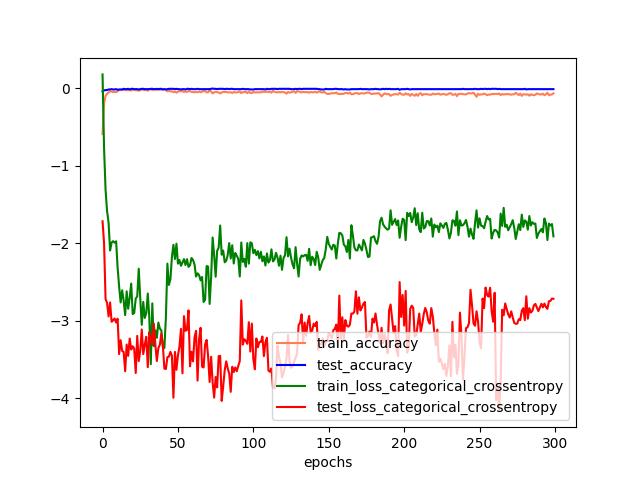
\includegraphics[width=0.49\textwidth]{graphs/model_2.png}
    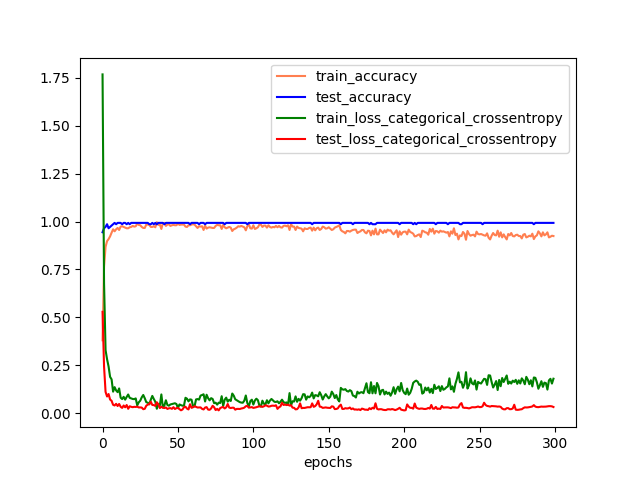
\includegraphics[width=\textwidth]{graphs/model_3.png}
    \caption{Modelele 1, 2 și 3}
\end{figure}

Acuratețea este foarte bună în cele 3 cazuri, însă nu se comportă atât de bine pe imagini noi, într-un mediu diferit.
De asemenea, am constatat ca luminozitatea și modul în care utilizatorul este plasat față de webcam sunt foarte importante și influențează performanța semnificativ.

Un lucru important de observat, care se va regăsi în majoritatea graficelor, sunt acele oscilații, alternanțe ale acurateței, care urcă și coboară.
Stratul \emph{Dropout} este cel care cauzează acest comportament, prin modul în care funcționează: ``by randomly dropping units during training to prevent their co-adaptation'', precum este menționat de \cite{dropout_algorithm}.
Acesta elimină neuroni ai unui strat, în mod aleatoriu, pentru a permite tuturor neuronilor să participe la învățare și să sporească performanța rețelei.
Astfel, atunci când sunt eliminați neuroni ``buni`'', adică aceia care conțin multă informație utilă pentru rezultatul final, performanța (acuratețea, eroarea) pot fi afectate negativ.
Pe de cealaltă parte, atunci când sunt eliminați neuroni care nu ajută foarte mult pentru predicție, performanța nu este afectata prea mult.

Am continuat prin a antrena aceeași rețea, pe o grilă de dimensiune 3x3, dar de data aceasta folosind toate imaginile disponibile.
Totuși, acest lucru nu a ajutat foarte mult și am observat și că după o anumită epocă, rețeaua nu se mai comporta bine pe datele de test și apărea fenomenul de \emph{overfit}.
Acest lucru se poate observa pe graficul modelului 4, unde acuratețea pentru datele de antrenament și cea pentru datele de testare încep să diveargă.

\begin{figure}[h]
    \centering
    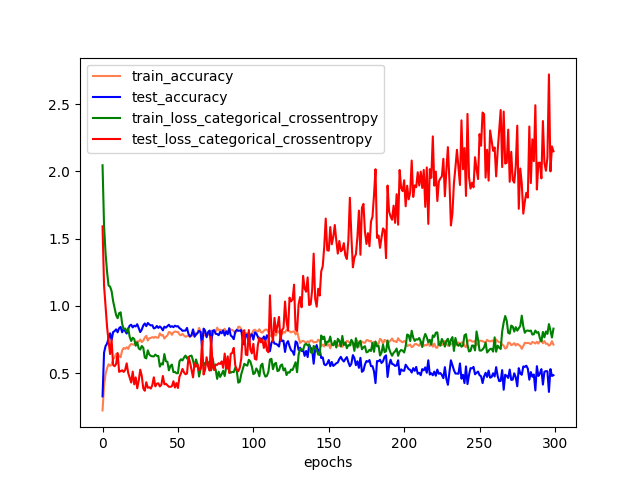
\includegraphics[width=0.66\textwidth]{graphs/model_4.png}
    \caption{Modelul 4}
\end{figure}

Pentru a rezolva problema overfit-ului, am introdus o \emph{regularizare L2} care, conform \cite{l1_l2_regularisation}, ar trebui să ajute în acest caz.
Într-adevăr, situația a fost ameliorată, însă nu a ajutat modelul să prezică mai bine zona în care mă uitam.

\begin{figure}[h]
    \centering
    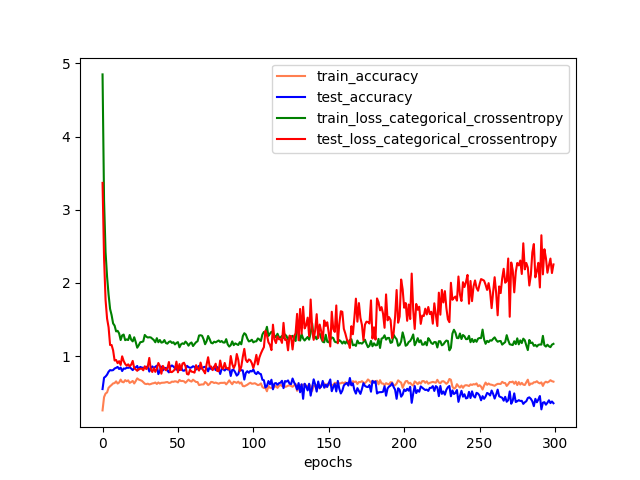
\includegraphics[width=0.49\textwidth]{graphs/model_5.png}
    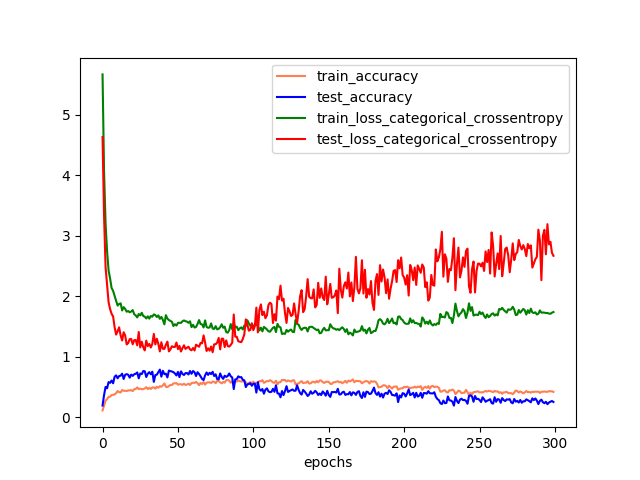
\includegraphics[width=0.49\textwidth]{graphs/model_6.png}
    \caption{Modelele 5 și 6}
\end{figure}

\section{Rețele neuronale de convoluție}
\subsection{Utilizarea întregii feți}

Mai departe am vrut să experimentez cu rețelele convoluționale și am început prin a utiliza fețele extrase din imagini\ref{fig_extracted_faces}, pe o grilă de dimensiune 2x2 \ref{grid-example}.
Din păcate, nu am avut rezultate deloc bune în primă fază.
După o analiză a codului și a datelor, am descoperit că aveam o problemă în cod și că datele nu erau normalizate, fapt care împiedica rețeaua din a învăța.
Am rezolvat această problemă și am continuat experimentarea.

Iată arhitectura cu care am obținut rezultatele ce urmează a fi prezentate:

\label{cnn_first_architecture}
\begin{lstlisting}[language=Python, caption=Prima arhitectură CNN]
model = Sequential()
model.add(Conv2D(16, kernel_size=(3, 3),
                    input_shape=input_shape))
model.add(MaxPooling2D(pool_size=(2, 2)))
model.add(ReLU())
model.add(Conv2D(32, kernel_size=(3, 3)))
model.add(MaxPooling2D(pool_size=(2, 2)))
model.add(ReLU())
model.add(Flatten())
model.add(Dense(128, activation='relu'))
model.add(Dense(4, activation='softmax'))
# optimizer used
opt = Adam()
\end{lstlisting}

\paragraph{Important}
Pentru primele experimente din această secțiune am folosit doar imaginile în care utilizatorul se uita în colțurile ecranului.
De exemplu, pentru o grilă de dimensiune 3x3, am ales doar imaginile în care eticheta corespunzătoare a imaginii este $0, 2, 6$ sau $8$.
Ultima mențiune este că datele de antrenament reprezintă $80\%$ din mulțimea totală de date, restul fiind date de testare.


Mai jos sunt parametrii de antrenare și rezultatele antrenării:

\begin{center}
    \begin{tabular}{ c | c | c | c | c | c | c }
        \hline
        Experiment & Dim. grilă & Nr. imagini & Epoci & Optimizatori & Rată de învățare & Batch size \\ 
        \hline
        7 & 2x2 & 2184 & 50 & Adam & 0.001 & 32 \\
        \hline
        8 & 3x3 & 1247 & 50 & Adam & 0.001 & 32 \\
        \hline
        9 & 4x4 & 711 & 50 & Adam & 0.001 & 32 \\
        \hline
    \end{tabular}
\end{center}

\begin{figure}[h]
    \centering
    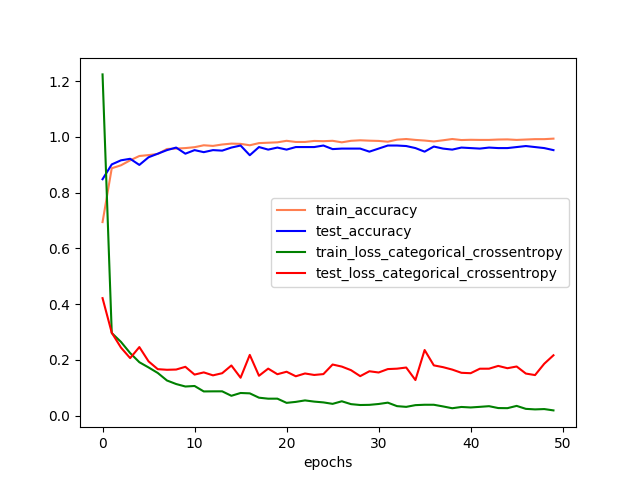
\includegraphics[width=0.32\textwidth]{graphs/model_7.png}
    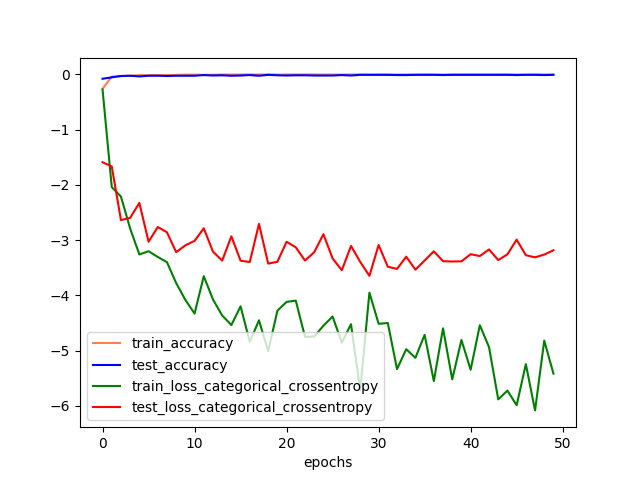
\includegraphics[width=0.32\textwidth]{graphs/model_8.png}
    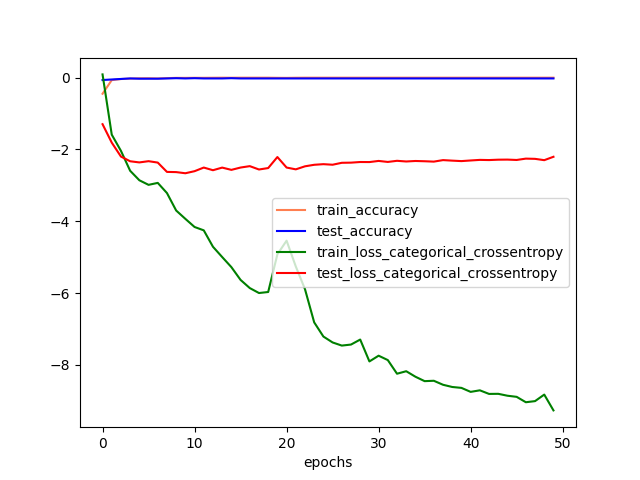
\includegraphics[width=0.32\textwidth]{graphs/model_9.png}
    \caption{Modelele 7, 8 și 9}
\end{figure}

Modelele 8 și 9 au performanțe bune, dar sunt instabile când le folosesc în condiții reale.
Modelul 7 s-a descurcat mai bine.
Dacă mă poziționez la un unghi prielnic față de cameră, acesta poate prezice destul de bine unde privesc.
Acest lucru este probabil datorat faptului că a fost antrenat folosind mai multe date.

Pentru experimentele 10 și 11, am adunat mai multe imagini și am antrenat aceeași arhitectură CNN pe toate datele (nu doar cele corespunzătoare colțurilor ecranului), ceea ce a însemnat 2736 de imagini, pentru grilele de dimensiune 3x3 și 4x4.
Rezultatele au fost mai bune, ceea ce m-a făcut să constat că performanța unui model crește direct proporțional cu dimensiunea mulțimii de date pe care o avem la dispoziție.
Putem vedea de asemenea semne de overfit în aceste modele.

\begin{figure}
    \centering
    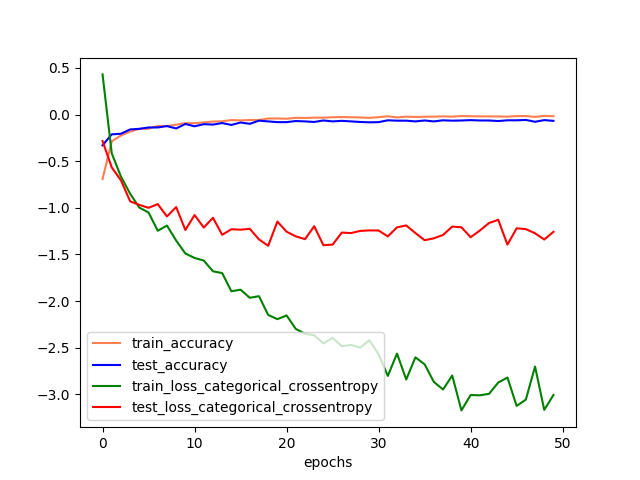
\includegraphics[width=0.49\textwidth]{graphs/model_10.png}
    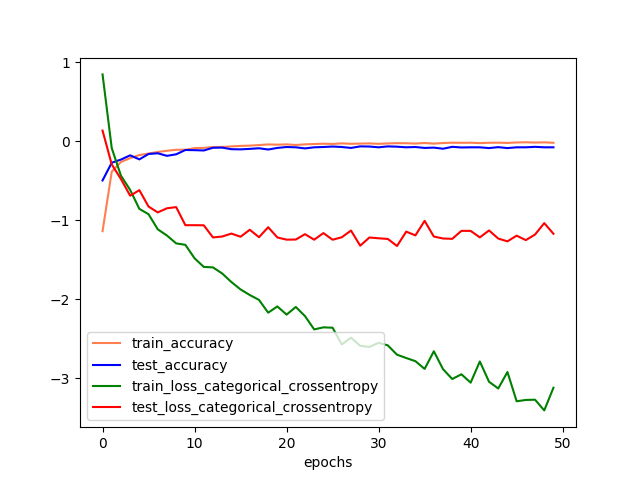
\includegraphics[width=0.49\textwidth]{graphs/model_11.png}
    \caption{Modelele 10 și 11}
\end{figure}

\subsection{Utilizarea ``benzilor oculare'' ca date de antrenament}
Am folosit aceeași arhitectură de rețea convoluțională ca mai sus, dar de această dată folosind doar porțiunile dreptunghiulare care încadrează ambii ochi\ref{fig_extracting_eye_strip}.
Primele modele au fost antrenate doar cu acele imagini în care utilizatorul se uita în colțurile ecranului.

\begin{center}
    \begin{tabular}{ c | c | c | c | c | c | c }
        \hline
        Experiment & Dim. grilă & Nr. imagini & Epoci & Optimizatori & Rată de învățare & Batch size \\ 
        \hline
        12 & 2x2 & 2184 & 50 & Adam & 0.001 & 32 \\
        \hline
        13 & 3x3 & 1247 & 50 & Adam & 0.001 & 32 \\
        \hline
        14 & 4x4 & 711 & 50 & Adam & 0.001 & 32 \\
        \hline
    \end{tabular}
\end{center}

\begin{figure}
    \centering
    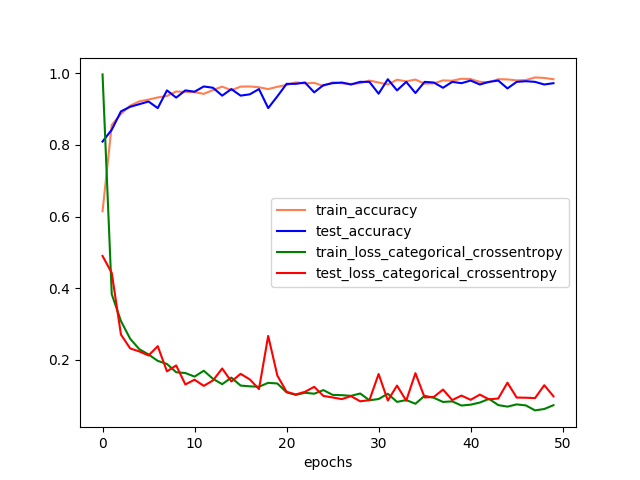
\includegraphics[width=0.32\textwidth]{graphs/model_12.png}
    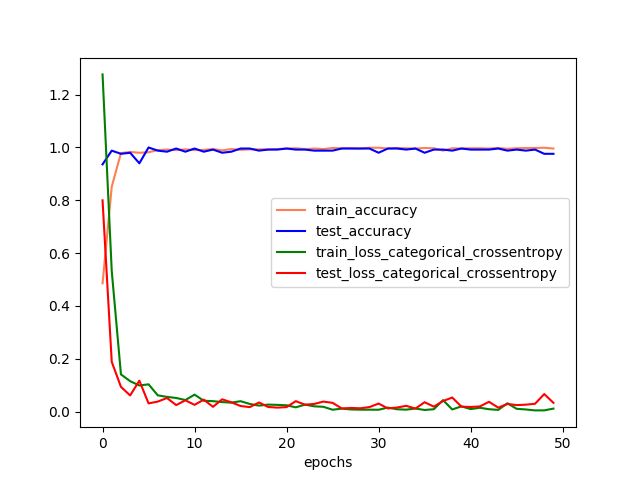
\includegraphics[width=0.32\textwidth]{graphs/model_13.png}
    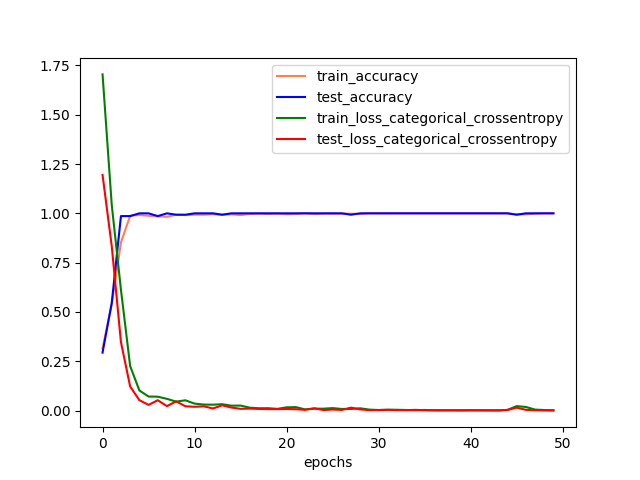
\includegraphics[width=0.32\textwidth]{graphs/model_14.png}
    \caption{Modelele 12, 13 și 14}
\end{figure}

Experimentul 12 a fost unul reușit.
În cadrul acestuia am putut prezice relativ bine unde mă uitam în condiții reale, chiar dacă mă indepărtam sau apropiam de ecran.

Am observat, de asemenea, aceeași tendință de scădere a performanței atunci când modelele sunt antrenate pe mai o mulțime de date mai mică, motiv pentru care experimentele 13 și 14 nu au fost atât de reușite în condiții reale.
Faptul acesta a fost confirmat, întrucât prezicerea a fost mai stabilă, dar tot nu era utilizabilă pentru un produs finit.

\begin{figure}
    \centering
    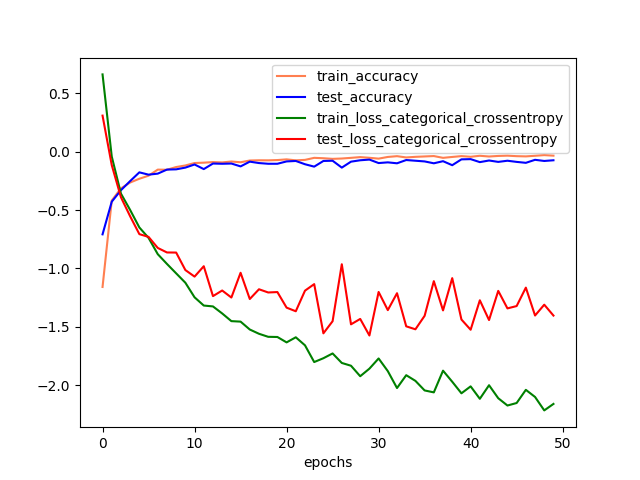
\includegraphics[width=0.49\textwidth]{graphs/model_15.png}
    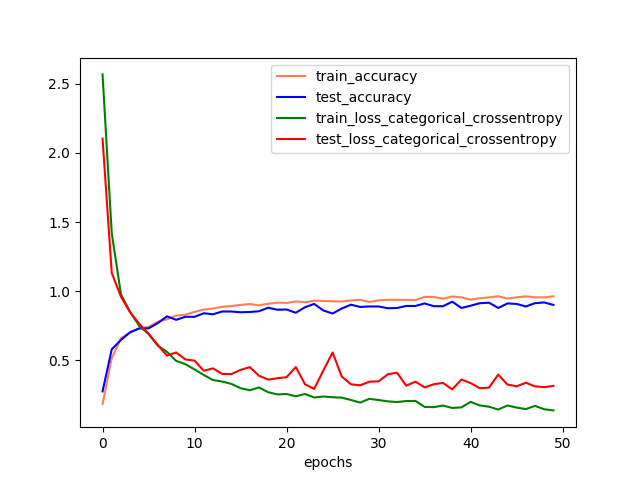
\includegraphics[width=0.49\textwidth]{graphs/model_16.png}
    \caption{Modelele 15 și 16}
\end{figure}

\paragraph{Comentariu intermediar}
Din experimentele prezentate până acum am concluzionat că cea mai bună variantă este folosirea rețelelor convoluționale împreună cu ``benzile oculare''.
Mai mult, atunci când am folosit același algoritm pe mai multe date, modelul realizat a fost mai stabil și a avut performanțe mai bune.
Acest fapt subliniază, din nou, importanța datelor într-un algoritm de învățare automată.

\subsection{Îmbunătățirea arhitecturii CNN}
Experimentele 17–22 au fost rezultatul încercării de a îmbunătăți arhitectura inițială a rețelei de convoluție pe care am folosit-o\ref{cnn_first_architecture}.
Am incercat fie să elimin straturi de convoluție, fie să schimb numărul filtrelor pentru a observa care este comportamentul acesteia.

Am remarcat că atunci când suprimez al doilea strat de convoluție, rețeaua nu mai poate spune atunci când mă uit la anumite celule, deși înainte nu avea probleme în acest sens (spre exemplu celula numărul 2, pe o grilă de dimensiune 3x3).
De asemenea, prin creșterea numărului de filtre de convoluție, performanța a crescut, așadar am decis să continui cu această arhitectură:

\begin{lstlisting}[language=Python, caption=Arhitectura CNN îmbunătățită]
model = Sequential()
model.add(Conv2D(64, kernel_size=(3, 3),
                    input_shape=input_shape))
model.add(MaxPooling2D(pool_size=(2, 2)))
model.add(ReLU())
model.add(Conv2D(128, kernel_size=(3, 3)))
model.add(MaxPooling2D(pool_size=(2, 2)))
model.add(ReLU())
model.add(Flatten())
model.add(Dense(128, activation='relu'))
model.add(Dense(Config.grid_size * Config.grid_size, activation='softmax'))
\end{lstlisting}

\section{Regresie folosind CNN}
O altă idee pe care am avut-o a fost să transform problema inițială, din clasificare în regresie.
Am încercat să prezic exact poziția (coordonatele) la care utilizatorul se uită, iar apoi să o traduc în numărul celulei corespunzătoare.

Pentru acest lucru, am adaptat arhitectura precedentă, astfel încât ultimul strat să fie format din doar 2 neuroni corespunzători coordonatelor (x, y) ale cursorului de pe ecran.
Am schimbat și funcția de activare de pe acest ultim strat într-o funcție liniară $f(x)=x$.
O altă schimbare necesară constă în definirea erorii.
Pentru această regresie am folosit \emph{eroarea medie pătratică} (\emph{Mean Squared Error}, abreviat MSE).
Astfel, formula de calcul a erorii devine:
$$
E = \frac{1}{n} * \sum_{i=1}^{n}{(\hat{y}_{i} – y_i)^2}
$$
unde $y$ este vectorul de coordonate reale (ceea ce trebuie să prezicem), iar $\hat{y}$ este vectorul rezultat, predicția modelului nostru.

Am introdus și o scădere treptată a ratei de învățare (learning rate decay), menită să ajute rețeaua să invețe mai mult și să conveargă mai precis spre parametrii optimi.
În cazul tehnologiei Keras pe care am folosit-o, rata de învățare se adaptează astfel:
\begin{center}
    \lstinline{lr = initial_lr * (1 / (1 + decay * iteration))}
\end{center}
Avantajul unei astfel de tehnici este că putem seta rata de învățare mai mare la început, pentru a invăța mai repede, apoi să o micșorăm pentru a face pași mai mici, dar mai preciși.
Metoda aceasta a dat rezultate pentru un număr mai mare de epoci și a rezultat într-un model care se descurca bine în a atinge obiectivul principal al acestei lucrări.

\begin{center}
    \begin{tabular}{ c | c | c | c | c | c | c }
        \hline
        Experiment & Dim. grilă & Nr. imagini & Epoci & Optimizatori & Rată de învățare & Batch size \\ 
        \hline
        22 & 3x3 & 2736 & 50 & Adam & 0.001 & 32 \\
        \hline
        23 & 3x3 & 2736 & 100 & \vtop{\hbox{\strut Adam}\hbox{\strut decay=$10^{-4}$}} & 0.001 & 32 \\
        \hline
        24 & 3x3 & 2736 & 100 & \vtop{\hbox{\strut Adam}\hbox{\strut decay=$10^{-4}$}} & 0.01 & 32 \\
        \hline
    \end{tabular}
\end{center}

\begin{figure}
    \centering
    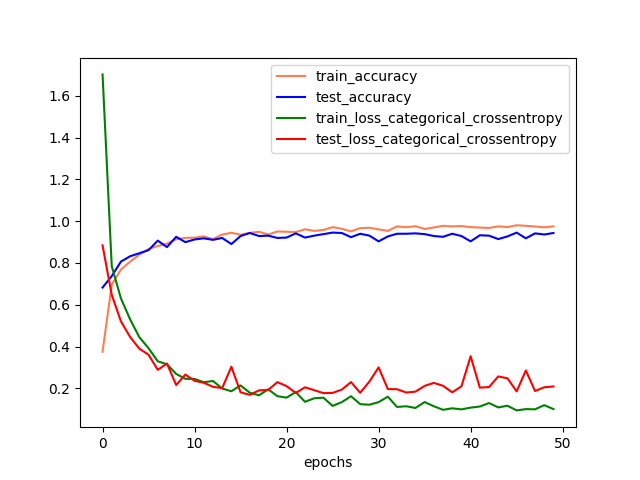
\includegraphics[width=0.32\textwidth]{graphs/model_22.png}
    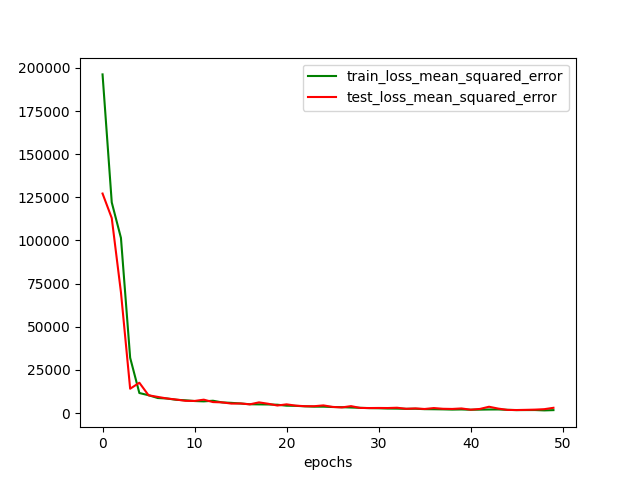
\includegraphics[width=0.32\textwidth]{graphs/model_23.png}
    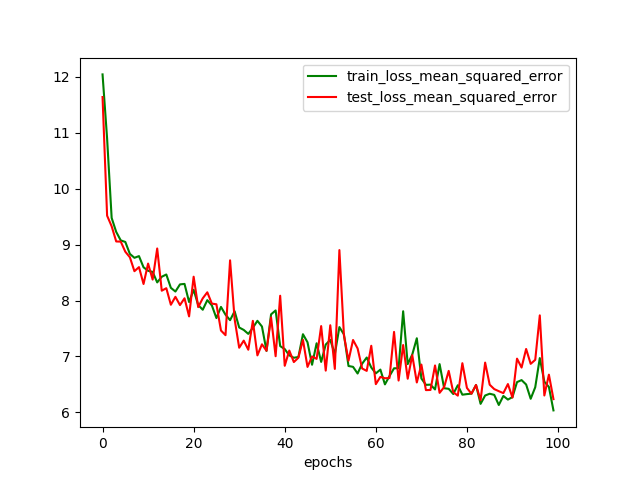
\includegraphics[width=0.32\textwidth]{graphs/model_24.png}
    \caption{Modelele 22, 23 și 24}
\end{figure}

\begin{figure}[h]
    \centering
    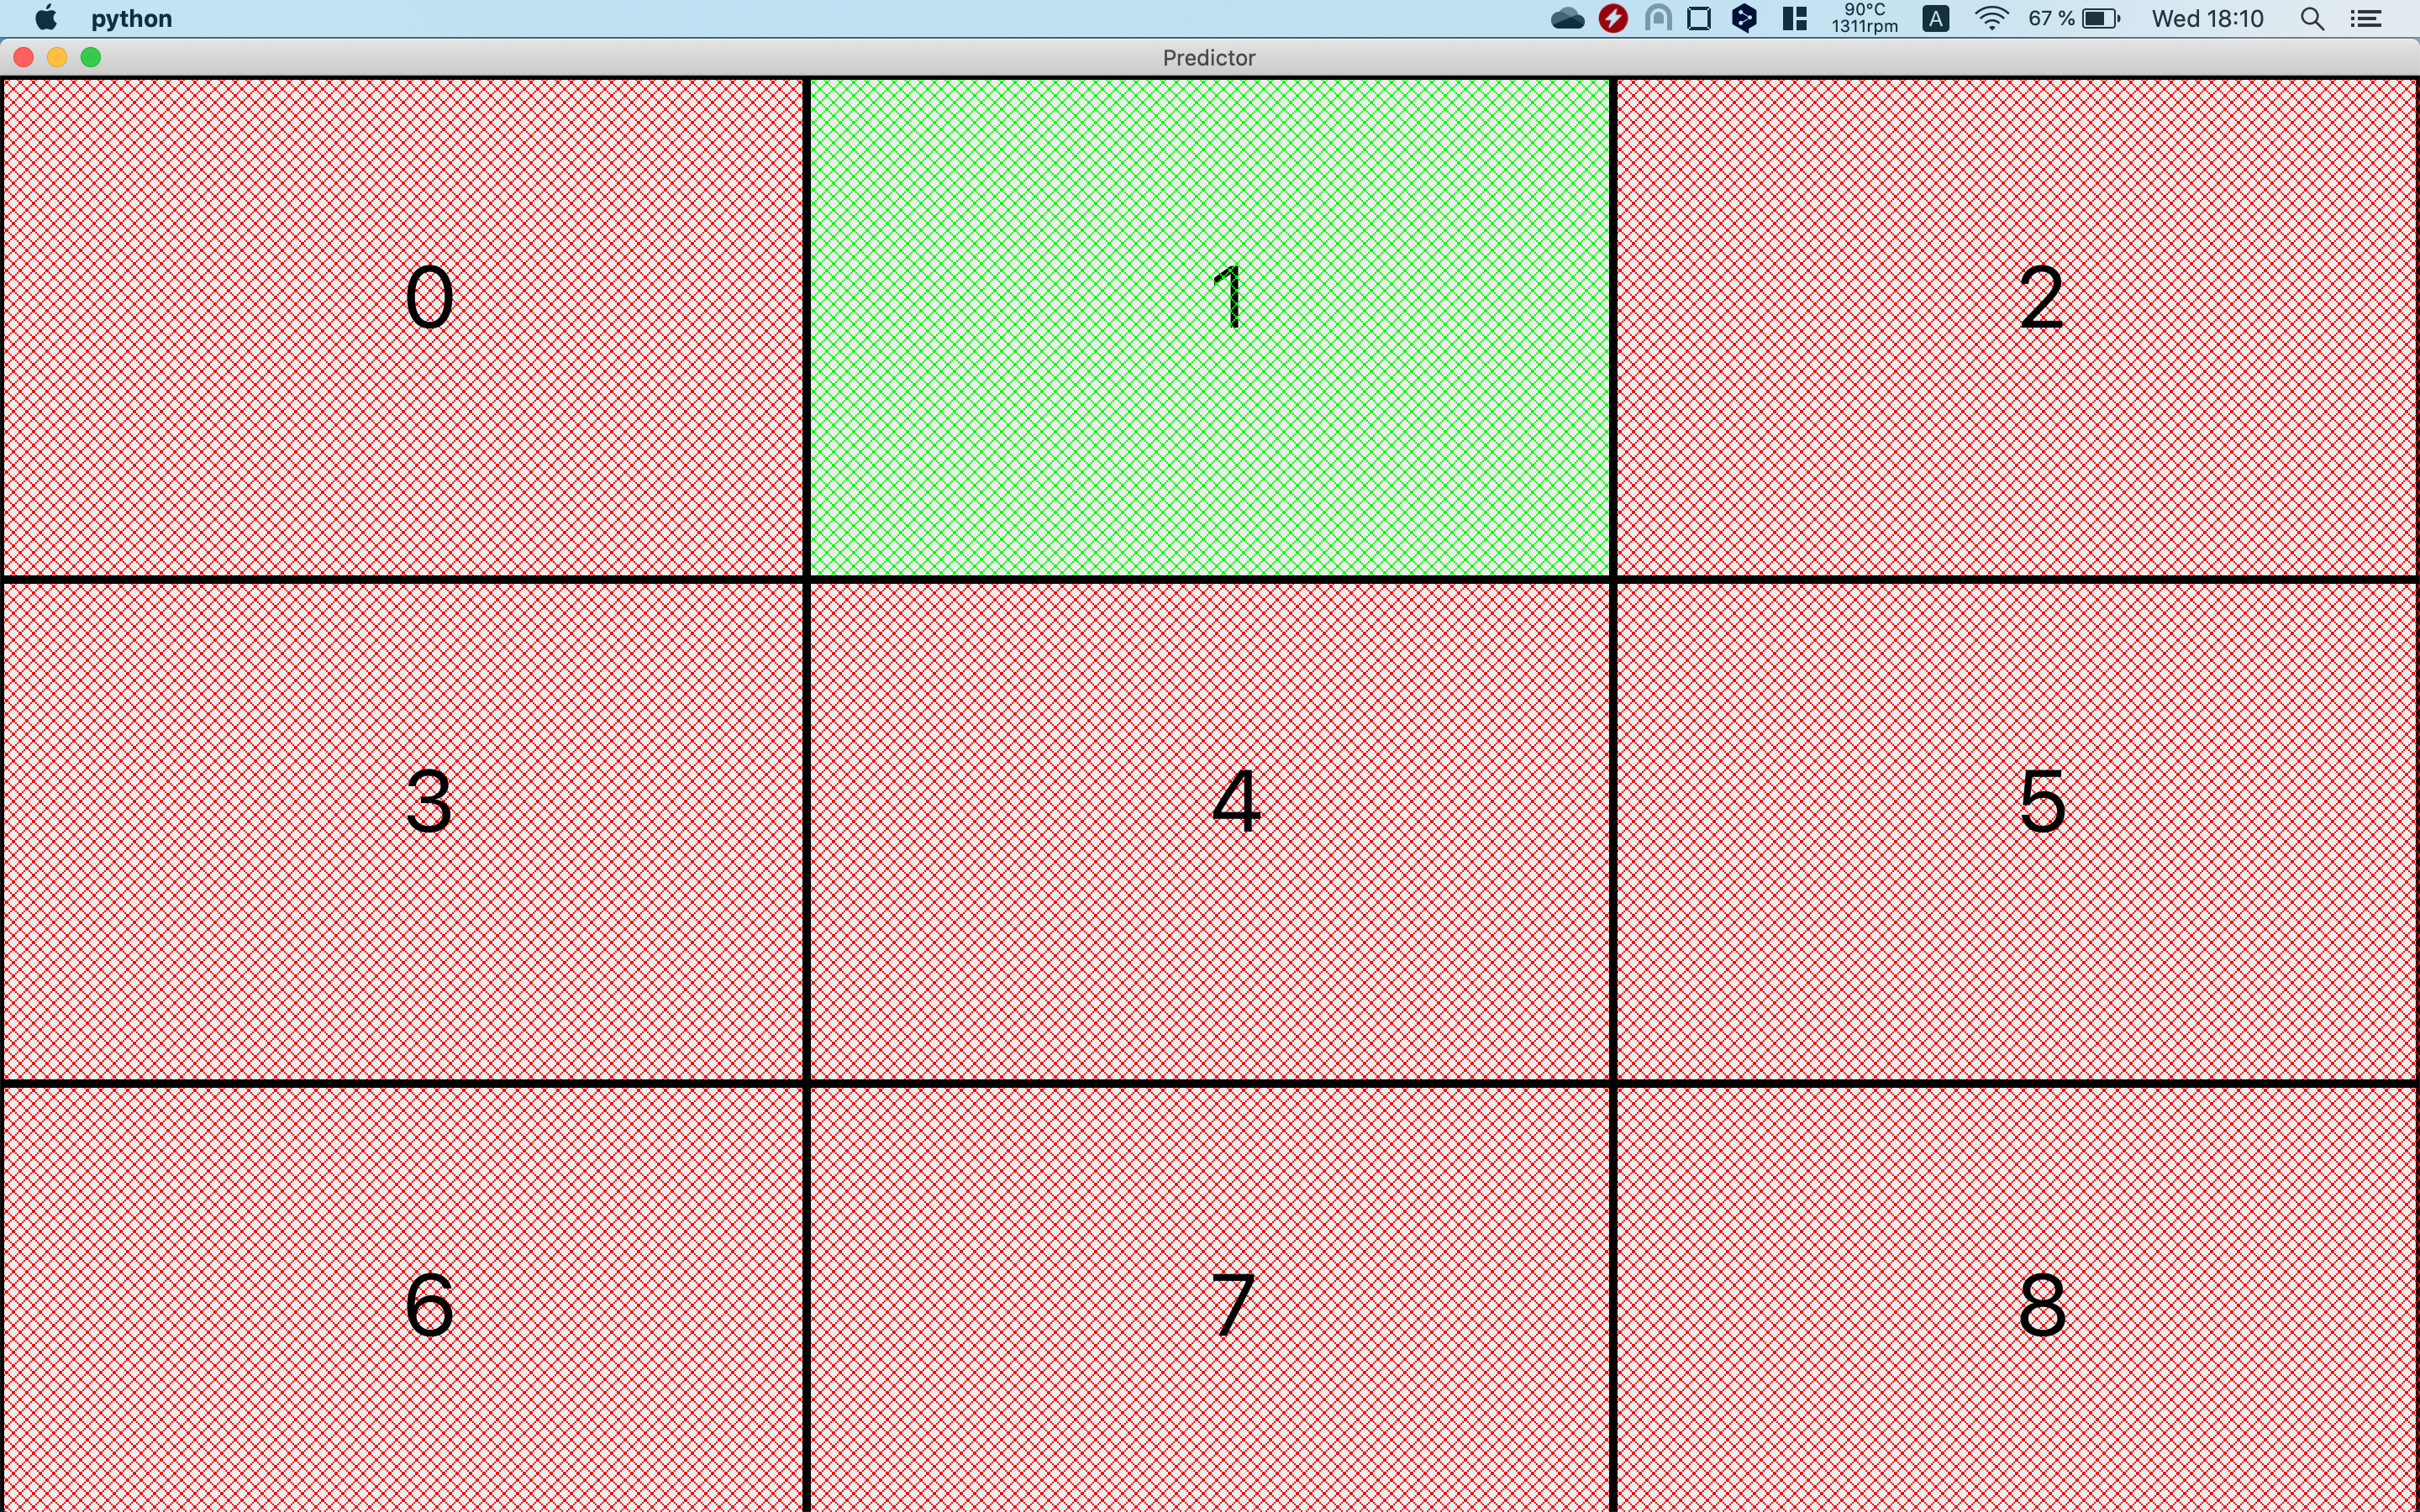
\includegraphics[width=0.49\textwidth]{pred1.png}
    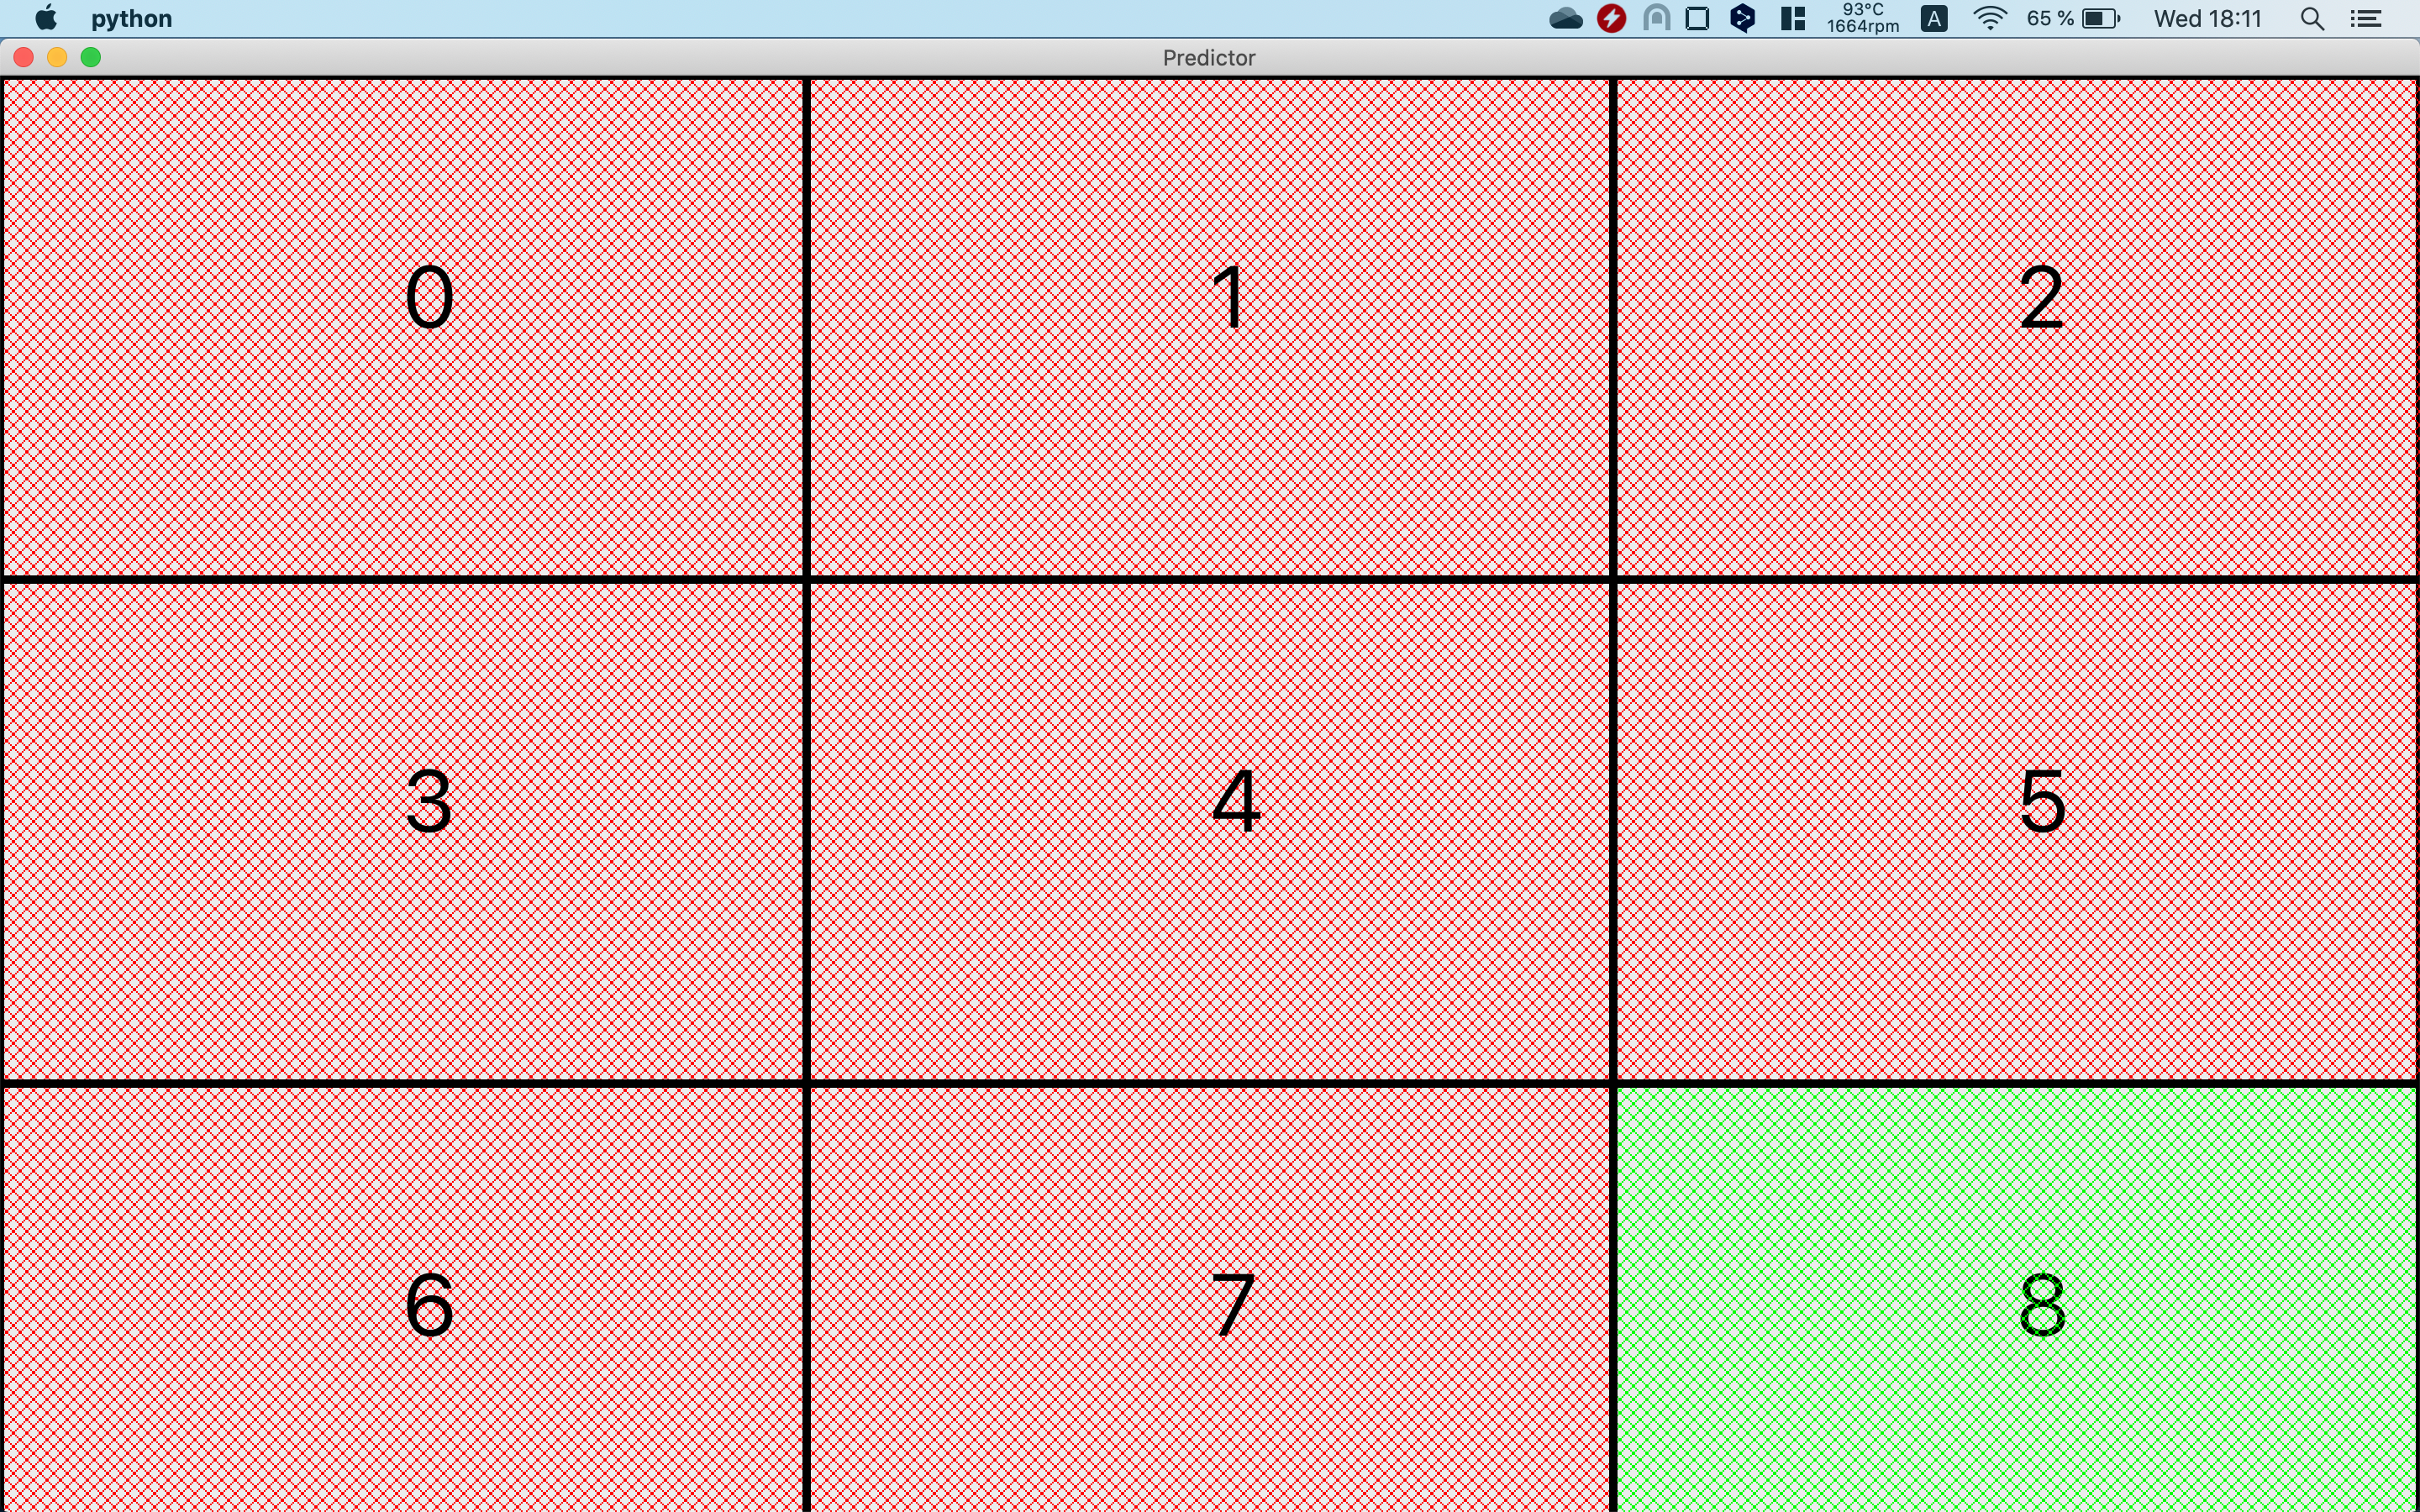
\includegraphics[width=0.49\textwidth]{pred2.png}
    \caption{Utilizarea rețelei CNN pentru urmărirea ochilor}
\end{figure}